\chapter{Resultados}

Na tabela \ref{estadoAtual} pode ser visualizado as Histórias de Usuário, a pontuação e o estado (a fazer, em progresso ou feito) de cada História. Foram implementados 12 pontos do total de 48 pontos estimados. Sendo assim, já foi implementado 25\% dos pontos da ferramenta InvestMVC.

\begin{table}[H]
\caption{Estado atual da ferramenta InvestMVC}
\begin{center}
    \begin{tabular}{ | c | c | c |}
    \hline
    \textbf{Histórias de Usuário} & \textbf{Pontuação} & \textbf{Estado} \\ \hline

US1 - Agente Correlação Linear & 3 & Em progresso\\ \hline
US2 - Agente Fibonacci & 3 & A fazer \\ \hline
US3 - Agente Mínimos Quadrados & 3 & A fazer\\ \hline
US4 -  Agente Tendência & 2 & Em progresso\\ \hline
US5 - Agente Gestor/Consultor & 2& Em progresso\\ \hline
US6 - Criar conta de usuário & 2 & Feito\\ \hline
US7 - Acompanhar retorno financeiro & 5 & A fazer\\ \hline
US8 - Criar Experts & 2 & Feito\\ \hline
US9 - Editar Experts & 2 & Feito\\ \hline
US10 - Excluir Experts & 2 & Feito\\ \hline
US11 - Ativar Expert & 1 & A fazer\\ \hline
US12 - Desativar Expert & 2 & A fazer \\ \hline
US13 - Método Correlação Linear em linguagem C & 2 & Feito\\ \hline
US14 - Método Fibonacci em linguagem C & 2 & Feito\\ \hline
US15 - Método Mínimos Quadrados em linguagem C & 2 & Feito\\ \hline
US16 - Método Correlação Linear em linguagem Haskell & 2 & Em progresso\\ \hline
US17 - Método Fibonacci em linguagem Haskell & 2 & Em progresso\\ \hline
US18 - Método Mínimos Quadrados em linguagem Haskell & 2 & Em progresso\\ \hline
US19 - Inserir na Base de Conhecimento & 2 & A fazer\\ \hline
US20 - Retirar na Base de Conhecimento & 2 & A fazer\\ \hline
US21 - Calcular Critério de Entrada & 3 & A fazer\\ \hline
US22 - Realizar Operação no MetaTrader& 1 & Feito\\ \hline
\end{tabular}
\end{center}
\label{estadoAtual}
\end{table}


\section{Resultados Testes Unitários}
\subsection{Componente Orientado a Objetos}
\subsection{Componente Funcional}
\textbf{Teste unitário paradigma funcional}

Foram realizados os testes unitários na linguagem haskell utilizando o framework HUnit. O framework não fornece a cobertura de código fonte, mas é possível visualizar a quantidade de casos de teste, quantidade de testes realizados, quantidade de erros e quantidade de falhas. Os resultados dos testes unitários dos métodos de Correlação de Pearson, Fibonacci e Mínimos Quadrados podem ser visualizados na figura \ref{testeCorrelacaoHaskell}, \ref{testeFibonacciHaskell} e \ref{TesteMinimosHaskell}.

\begin{figure}[H]
\centering
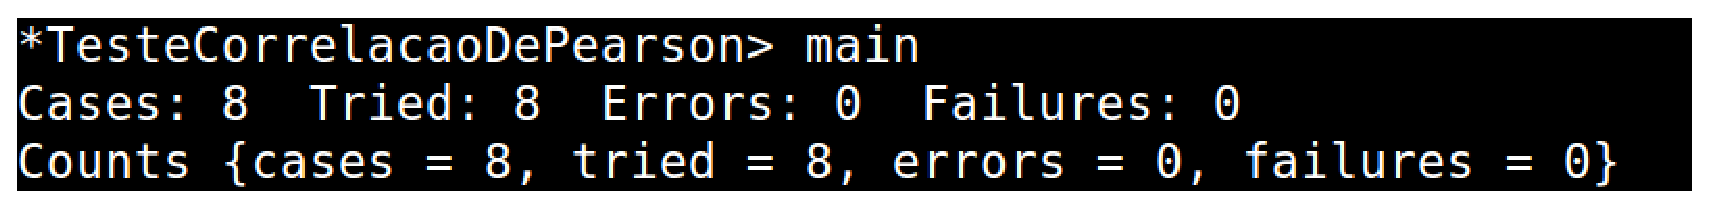
\includegraphics[width=0.9\textwidth]{figuras/testeCorrelacaoHaskell}
\caption{Resultado da Suíte de Teste do Método Correlação Linear}
\label{testeCorrelacaoHaskell}
\end{figure}

\begin{figure}[H]
\centering
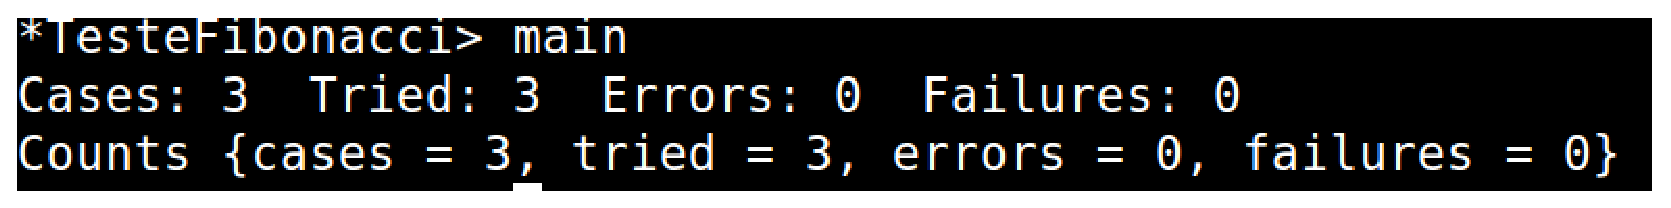
\includegraphics[width=0.9\textwidth]{figuras/testeFibonacciHaskell}
\caption{Resultado da Suíte de Teste do Método de Fibonacci}
\label{testeFibonacciHaskell}
\end{figure}

\begin{figure}[H]
\centering
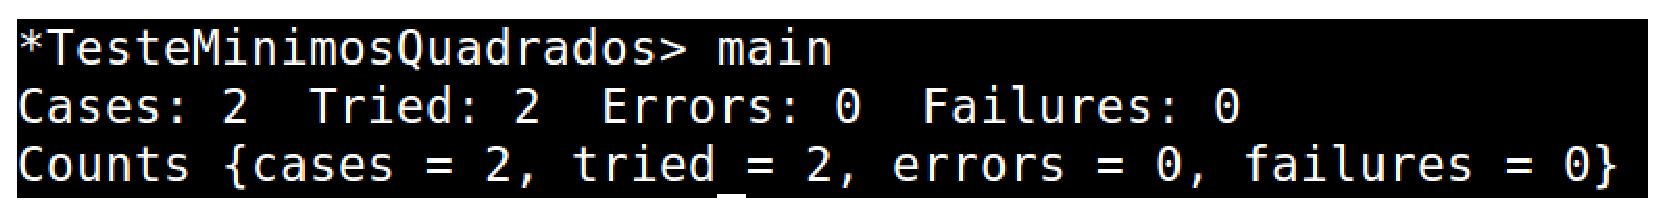
\includegraphics[width=0.9\textwidth]{figuras/TesteMinimosHaskell}
\caption{Resultado da Suíte de Teste do Método Mímimos Quadrados}
\label{TesteMinimosHaskell}
\end{figure}


\subsection{Componente Estruturado}

\subsection{Componente Multiagente}

\subsection{Componente Lógico}
